\documentclass[11pt]{article}

\usepackage[margin=1.1in]{geometry}
\usepackage{booktabs}
\usepackage{array}
\usepackage{graphicx}
\usepackage{amsmath}
\usepackage{microtype}
\usepackage[table]{xcolor}
\usepackage[colorlinks=true,linkcolor=black,citecolor=black,urlcolor=blue!55!black]{hyperref}
\usepackage{caption}
\captionsetup{font=small,labelfont=bf}

\usepackage{titlesec}
\titleformat{\section}{\normalfont\large\bfseries}{\thesection}{0.6em}{}
\titleformat{\subsection}{\normalfont\normalsize\bfseries}{\thesubsection}{0.6em}{}

\newcommand{\tw}[1]{\texttt{\small #1}}

\title{\bfseries What You Are Actually Measuring When You\\Benchmark Speculative Decoding Under FP8}

\author{%
  Akshath Tiwari\\
  \small Independent\\
  \small \href{mailto:tiwariakshath@gmail.com}{tiwariakshath@gmail.com}
}
\date{\today}

\begin{document}
\maketitle

\begin{abstract}
\noindent
Speculative decoding and FP8 quantization are both standard in production
LLM serving, and their interaction is almost always reported from single
runs. We set out to measure that interaction on Ada-class hardware and
could not, four times, until the measurement apparatus itself was fixed.

We identify and quantify four confounds on vLLM 0.29.0 / NVIDIA L4 (SM89).
First, attention-backend selection is \emph{conditioned on KV-cache dtype},
so an FP8-versus-BF16 comparison under default settings silently swaps the
attention kernel as well; target and draft models select backends
independently, so pinning one does not pin the other. Second, speculative
throughput is \emph{bimodal across boots} of an identical configuration,
varying up to $2.96\times$ while acceptance does not; the mode is selected
by the CUDA-graph execution path and fixed at boot. Third, the acceptance
rate $\tau$ has a \emph{boot-to-boot noise floor of 1.32\%} that no prior
work reports, below which ``precision does not affect acceptance'' claims
are unfalsifiable and above which small effects have been reported as real.
Fourth, the metric universally called \emph{inter-token latency is
inter-chunk latency}: a speculative step emits every accepted token in one
stream chunk, so the measured gap exceeds the true per-token interval by
roughly~$\tau$.

The first three add error; the fourth reverses the ranking. Under a standard
p95-ITL service objective, every speculative configuration we measured
scores \emph{zero goodput at concurrency 64 while producing the most tokens
per second in the grid}. We report FP8~$\times$~speculative results with all
four controlled, and release the harness, the raw records, and the full
history of our own corrections --- seven retractions, each traceable to the
same error shape.
\end{abstract}

\section{Introduction}

Speculative decoding trades a small draft model's cheap guesses against the
target model's expensive verification~\cite{leviathan2023,chen2023}. Its
benefit is governed almost entirely by one quantity: $\tau$, the mean number
of tokens accepted per verification step. FP8 quantization independently
reduces weight and KV-cache footprint, which matters because KV capacity is
what binds under concurrency~\cite{kwon2023}. Serving stacks ship both. The
obvious question --- does quantization degrade acceptance, and what does the
combination buy under load --- is asked frequently and answered from
single-run measurements.

We could not answer it. Four separate times, a result we were about to
report turned out to be produced by something other than the variable under
study. This paper reports those four things, because they are larger than
the effect they obscured.

\paragraph{Contributions.}
\begin{enumerate}\itemsep2pt
\item \textbf{Backend substitution under dtype change} (\S\ref{sec:c1}).
vLLM's \tw{auto} backend selection is conditioned on KV-cache dtype, and
target and draft select independently. A precision A/B under defaults is a
kernel A/B as well.
\item \textbf{Bimodal speculative throughput} (\S\ref{sec:c2}). Identical
configurations boot into a fast or slow mode and stay there. We localise
this to \emph{draft-model} speculation: n-gram speculation shows no such
behaviour across twelve boots. \tw{-{}-enforce-eager} removes the
bimodality but is not a free control --- it costs FP8-weight configurations
a fifth to a half of their throughput and cannot boot speculative FP8-KV
cells at all on this card.
\item \textbf{The acceptance noise floor} (\S\ref{sec:c3}). $\tau$
reproduces to 1.32\% across boots. We report FP8's effect on $\tau$ as
bounded \emph{below} that floor rather than as a null result, and withdraw
one of our own earlier claims that sat at $1.7\times$ the floor.
\item \textbf{ITL is inter-chunk latency} (\S\ref{sec:c4}). A speculative
step emits every accepted token in one stream chunk, so a p95-ITL objective
ranks the highest-throughput configuration in the grid as fully
non-compliant. This one does not add error --- it inverts the decision.
\item \textbf{Results with all four controlled} (\S\ref{sec:results}):
compatibility, KV capacity, task accuracy at $n{=}256$, and goodput.
\item \textbf{A fully auditable artifact} (\S\ref{sec:artifact}):
append-only raw records, script-regenerated derived tables, provenance
checked by a script that fails the build, and every retraction preserved
rather than removed.
\end{enumerate}

We emphasise the last because it is what made the others findable. Most of
our corrections were caught by re-reading stored records against a
hypothesis formed later --- impossible if results are summarised at write
time.

\section{Setup}\label{sec:setup}

\begin{table}[h]\centering\small
\begin{tabular}{ll}
\toprule
Engine & vLLM 0.29.0, pinned; version read from the running server over HTTP\\
GPU & NVIDIA L4 (SM89, Ada, 24\,GB nominal / 22.03\,GiB usable), rented per second\\
Target & Qwen3-4B\\
Draft & \tw{z-lab/Qwen3-4B-DFlash-b16}, block size 16, 5 speculative tokens\\
Also & n-gram (prompt-lookup) speculation, no draft checkpoint\\
Workload & GSM8K~\cite{cobbe2021}, sampled without replacement\\
Base image & \tw{nvidia/cuda:13.0.3-devel-ubuntu24.04}\\
\bottomrule
\end{tabular}
\end{table}

\noindent
L4 was chosen deliberately: it is the compute capability named in the
upstream reports that motivated the study, and at 22\,GiB the KV-capacity
constraint actually binds, which it does not on an 80\,GB card.

\paragraph{The harness never imports the engine.} It launches vLLM as a
subprocess and speaks HTTP. This costs some convenience and buys the
guarantee that what we measure is what a serving deployment runs, not an
in-process configuration no server would produce.

\paragraph{Every measurement is content-addressed.} A configuration hashes
to a \tw{cell\_id}; identical configuration yields an identical id on any
machine. Records are append-only, so a re-run supersedes rather than
overwrites and the superseded record remains readable. Several of our
corrections depend on that history being intact.

\paragraph{Definition.} We define
\[
\tau \;=\; 1 + \frac{\text{accepted draft tokens}}{\text{verification steps}}.
\]
The $+1$ is the bonus token, which vLLM's counter excludes. Omitting it
understates $\tau$ by exactly 1 and silently changes every speedup ratio
derived from it.

\section{Confound 1: the attention backend moves when the dtype moves}\label{sec:c1}

vLLM's \tw{auto} attention-backend selection is a function of KV-cache
dtype. At BF16 KV it selects FlashAttention-2; at \tw{fp8\_e4m3} it selects
FlashInfer. An experimenter varying only precision therefore varies the
attention kernel too, and any resulting difference is jointly attributable.

It is worse than one substitution. Target and draft models select backends
\emph{independently}, at two distinct call sites, so pinning the backend
affects the target while the draft continues to select on its own. A
pinned-backend precision comparison is still confounded on the draft side
for speculative cells, which we record per cell rather than assert away.

Compatibility is not uniform. Of the four attention backends vLLM 0.29.0
offers on SM89, FP8 KV runs on exactly two.

\begin{table}[h]\centering\small
\caption{FP8 KV cache support by attention backend, Qwen3-4B + DFlash, SM89.
\tw{launch\_failed} is rejection at configuration time.}
\begin{tabular}{llr}
\toprule
Backend & FP8 KV status & KV tokens\\
\midrule
FLASHINFER & ok & 115{,}920\\
TRITON\_ATTN & ok & 129{,}584\\
FLASH\_ATTN & launch\_failed & ---\\
FLEX\_ATTENTION & launch\_failed & ---\\
\tw{auto} & ok (selects FLASHINFER) & 115{,}920\\
\bottomrule
\end{tabular}
\end{table}

\noindent
This is the mechanism behind the dtype-conditioned selection: \tw{auto} does
not switch away from FlashAttention-2 under FP8 KV as a preference, it
switches because FlashAttention-2 \emph{cannot} serve FP8 KV on this
hardware. The original hypothesis motivating this study --- that FlashInfer's
FP8 attention kernels are SM90-only, so FP8 KV plus non-causal drafting
would crash on Ada --- is refuted. The combination runs.

\paragraph{Our own error here.} We initially concluded that the backend
selection flag was accepted, echoed back, validated against, and then
ignored, and reported this upstream. That was wrong: the flag controls the
target, and what we observed was the draft selecting independently. We
corrected the report. The mistake is instructive because we compared
requested-versus-selected backend for \emph{a server} when there is no such
thing as a server's backend --- there are two.

\section{Confound 2: speculative throughput is bimodal across boots}\label{sec:c2}

Booting an identical speculative configuration repeatedly produces
throughput in two clusters, not a spread. Acceptance is unchanged
throughout, so this is the cost of producing accepted tokens rather than how
many are accepted.

\begin{figure}[h]\centering
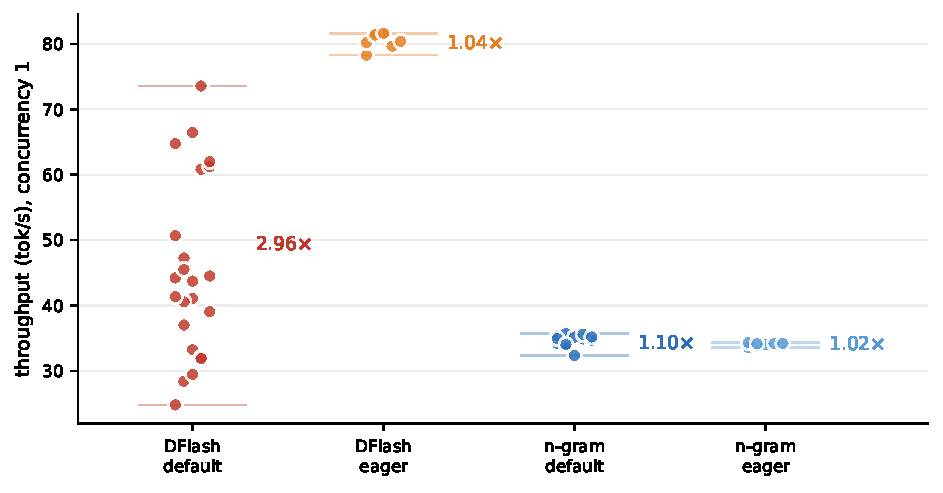
\includegraphics[width=0.86\textwidth]{figures/bimodality.pdf}
\caption{One dot per boot of an identical configuration at concurrency 1.
DFlash's default arm separates into two clusters with empty space between
them; n-gram's arms are single tight groups. A standard deviation cannot
distinguish these cases, and reading the first as continuous variance is
the error we originally made.}
\label{fig:bimodality}
\end{figure}

\paragraph{The selector is the CUDA-graph path.} vLLM emits, at every
speculative boot, a warning that \tw{CUDAGraphMode.FULL\_AND\_PIECEWISE} is
unsupported with spec-decode for the FlashInfer backend, and falls back.
Pinning \tw{cudagraph\_mode: PIECEWISE} reproduces the slow mode exactly
(30.04 versus 30.57 tok/s), indicating the fallback \emph{is} the slow mode
rather than a third state. Disabling CUDA graphs selects the fast mode
reliably.

\paragraph{The sharpest instance.} One content-addressed cell
(\tw{dflash\,|\,bf16\,|\,fp8\_e4m3\,|\,FLASHINFER}, graphs on) was measured
in two ordinary grid runs:

\begin{table}[h]\centering\small
\begin{tabular}{lrrr}
\toprule
Session & measurements (tok/s) & mean & $\tau$\\
\midrule
grid 1 & 28.59,\; 29.39,\; 33.81 & 30.60 & 4.183\\
grid 2 & 64.89,\; 71.77 & 68.33 & 4.211\\
\midrule
\multicolumn{2}{l}{ratio} & \textbf{2.23$\times$} & 0.68\% apart\\
\bottomrule
\end{tabular}
\end{table}

\noindent
Same \tw{cell\_id}, therefore the same configuration by construction, and a
matching \tw{argv} fingerprint. The $\tau$ difference of 0.68\% is
\emph{below} its own noise floor (\S\ref{sec:c3}). Every earlier
demonstration of this effect compared \emph{something} --- different arms,
different cells, boots inside a test built to show it. This compares nothing.

\paragraph{We report no speedup ratio from this effect.} Measuring both arms
inside a single run, with the default boot landing in the \emph{fast} mode,
gives $1.13\times / 1.06\times / 1.05\times$ at concurrency 1/16/64. Against a
slow-mode boot the same eager numbers give $2.19\times$. The ratio is a
statement about which mode the comparison arm drew, not about the flag. What
is stable is the \emph{spread}: two boots of an identical configuration
differ by $1.64\times$ at concurrency 16 under defaults and by $1.07\times$
with graphs off. Turning CUDA graphs off does not reliably make speculative
decoding faster --- it makes it \emph{measurable}, and whatever throughput it
gains is the slow-mode boots thereby avoided.

Our first write-up of this section led with $2.38\times$, obtained by
comparing against an arm we assumed representative, which was one draw from
the bimodal distribution this same section describes.

\paragraph{It is specific to draft-model speculation.} Running the identical
protocol with n-gram (prompt-lookup) speculation finds no bimodality across
twelve boots --- spread $1.10\times$ against DFlash's $2.96\times$ --- and no
benefit from \tw{-{}-enforce-eager} ($1.00\times$). These are the same fact
arriving twice: if there is no slow mode, there is nothing for the flag to
avoid. As a measurement sanity check, n-gram's acceptance is deterministic
($\tau = 1.732$ on every boot, spread $1.000\times$) where DFlash's moves
4.09--4.43, which is what a prompt-matching mechanism should do.

Twelve boots cannot prove absence. Pooling our DFlash default-arm boots
gives $P(\text{slow}) \approx 0.38$, so twelve draws land all-fast about
0.3\% of the time. We report this as a localisation, not an exclusion. The
consequence is that a claim like ours has to name the mechanism:
``speculative throughput is bimodal'' would be refuted by the first reader
who tries prompt-lookup.

\section{Confound 3: acceptance has a noise floor nobody had measured}\label{sec:c3}

$\tau$ reproduces to \textbf{1.32\%} across boots of an identical
configuration with identical prompts (4.0913--4.1452 over four boots). This
number did not exist before we measured it, and its absence had consequences
in both directions.

\paragraph{Permissive direction.} We had reported that $\tau$ is invariant to
FP8 precision, measuring a 0.7\% difference. With the floor known, the
correct statement is stronger and more precise: \emph{no effect larger than
1.3\% is detectable}, and the observed 0.7\% sits below it. A null result
becomes a bounded one.

\paragraph{Restrictive direction.} We had also reported that backend choice
perturbs $\tau$ more than precision does, citing a 2.25\% spread across four
backends. That is $1.7\times$ the noise floor, from single boots. It is not
separable from noise, and we withdraw it.

That claim moved three times before anyone measured the floor: asserted,
withdrawn for a wrong reason, restored, and now withdrawn for a sound one.
The reason it kept moving is that every argument about it was about the
effect and none was about the floor. One four-boot run settled it
permanently and cost about an hour of GPU time.

\paragraph{Prescription, and prior credit.} Measure the noise floor of the
quantity being compared \emph{before} comparing it.

We do not claim this principle as novel. Kaplan~\cite{kaplan2026calibrated},
concurrently, calibrates an LLM judge by scoring ``two ordinary runs of a
model given the same prompts'' and includes a null condition ``provably
identical in distribution\ldots whose measured difference must be zero''.
That is the same epistemic move. His instrument is an LLM judge and his
quantity is output quality; ours is a serving harness and our quantities are
acceptance and throughput. Independent concurrent arrival at the same
principle in adjacent subfields is evidence the principle is right, and we
cite it as such.

What we add is narrower and specific: \emph{the floor for $\tau$ had not been
measured}, and effects below it have been reported as real.

\paragraph{A caveat on the floor itself.} Our 1.32\% is measured at
$\tau \approx 4.1$, on GSM8K with a 768-token budget. In an earlier phase,
with a 256-token budget on a different prompt set, the same configuration
gave $\tau \approx 2.71$ --- a 55\% difference from generation length and
prompt distribution alone. A floor measured at one operating point should not
be transplanted to another, and $\tau$ quoted without its generation length
and prompt distribution is close to uninterpretable.

\section{Confound 4: ``inter-token latency'' is inter-chunk latency}\label{sec:c4}

The first three confounds add error. This one reverses the ranking.

A streaming client measures the gap between \emph{arrivals}. vLLM emits one
SSE chunk per decoding step, and a speculative verification step emits every
accepted draft token at once. So the quantity universally called inter-token
latency is \emph{inter-chunk} latency, and on a speculative server it
exceeds the true per-token interval by roughly $\tau$.

\begin{table}[h]\centering\small
\caption{Concurrency 64, CUDA graphs on, FP8 weights, auto KV, identical
prompts and SLO.}
\begin{tabular}{lrrrr}
\toprule
& measured gap & tokens/chunk & implied per-token & throughput\\
\midrule
speculative (DFlash) & \textbf{93.8\,ms} & \textbf{4.122} & \textbf{22.8\,ms} & \textbf{2219 tok/s}\\
non-speculative & 33.8\,ms & 1.007 & 33.6\,ms & 1281 tok/s\\
\bottomrule
\end{tabular}
\end{table}

\noindent
Speculation is $1.5\times$ faster per token and appears $2.8\times$ slower on
the metric. The \tw{tokens\_per\_chunk} of 4.122 tracks the measured $\tau$
of ${\approx}4.2$, as it must.

\begin{table}[h]\centering\small
\caption{Goodput at p95 ITL $\le$ 50\,ms, TTFT $\le$ 1000\,ms, concurrency 64.}
\begin{tabular}{lrrr}
\toprule
Configuration & raw req/s & SLO met & goodput req/s\\
\midrule
dflash\,|\,fp8\,|\,auto & \textbf{8.31} & \textbf{0\%} & \textbf{0.000}\\
dflash\,|\,bf16\,|\,auto & 6.13 & 0\% & 0.000\\
none\,|\,fp8\,|\,auto & 5.20 & 100\% & \textbf{5.188}\\
none\,|\,bf16\,|\,auto & 3.37 & 6\% & 0.209\\
\bottomrule
\end{tabular}
\end{table}

\noindent
Every speculative configuration scores zero goodput while producing the most
tokens in the grid. The fastest system is ranked last.

This is not an engine defect or a bug in our harness: a server cannot deliver
four tokens at four separate times when it produced them at one time. Any
client measuring arrival gaps, on any engine, sees this. At concurrency 1 the
effect is present but does not bite --- gaps are small in absolute terms and
speculative cells meet the same target 100\% of the time. It appears exactly
where serving operates.

We do not claim the quotient is the right metric. Dividing by
\tw{tokens\_per\_chunk} recovers a sensible average and discards the
burstiness an ITL target exists to capture; whether a reader perceives four
tokens every 94\,ms as smoother than one every 34\,ms is a question we did
not study. Our claim is narrower and sufficient: the metric as universally
computed does not measure what its name says under speculation, and using it
to gate a speculative deployment inverts the decision. Prior work
(\S\ref{sec:related}) reports single-request latency, where the effect does
not bite --- consistent with it going unreported.

\section{Results with all four controlled}\label{sec:results}

\subsection{The execution-path flag is not a free control}

We ran the full grid twice, 16 boots each, in independent containers, with
\tw{enforce\_eager} as an \emph{axis} rather than a pinned setting. Ratios
are graphs-off over graphs-on, so below 1.0 means eager is slower.

\begin{table}[h]\centering\small
\caption{Effect of \tw{-{}-enforce-eager}, two independent grids.}
\begin{tabular}{llrr}
\toprule
Configuration & conc & grid 1 & grid 2\\
\midrule
none\,|\,bf16\,|\,auto & 1 & 0.95$\times$ & 0.96$\times$\\
none\,|\,bf16\,|\,auto & 64 & 0.96$\times$ & 0.96$\times$\\
none\,|\,\textbf{fp8}\,|\,auto & 1 & \textbf{0.49$\times$} & \textbf{0.68$\times$}\\
none\,|\,\textbf{fp8}\,|\,auto & 64 & \textbf{0.66$\times$} & \textbf{0.78$\times$}\\
none\,|\,\textbf{fp8}\,|\,fp8\_e4m3 & 1 & \textbf{0.50$\times$} & \textbf{0.66$\times$}\\
dflash\,|\,bf16\,|\,auto & 1 & 1.13$\times$ & 1.32$\times$\\
dflash\,|\,\textbf{fp8}\,|\,auto & 1 & \textbf{0.61$\times$} & \textbf{0.76$\times$}\\
\bottomrule
\end{tabular}
\end{table}

\noindent
\tw{-{}-enforce-eager} costs FP8-weight configurations a fifth to a half of
their throughput and costs BF16 essentially nothing. Individual boots do not
overlap on any FP8 row and overlap on every BF16 row, in both grids. $\tau$
is unmoved throughout.

The direction replicates on every cell; the coefficient does not, and that
is itself a result. The graphs-on arm reproduces everywhere
(0.95--1.06$\times$), the eager arm reproduces for BF16 (1.00--1.05$\times$)
and does not for FP8 weights (1.22--1.40$\times$). The eager+FP8 arm is
boot-unstable --- tight within a boot (20.2 and 20.5 tok/s on grid 1's two
repeats) and $1.4\times$ between them.

This study therefore found \emph{two} unstable dimensions, each with a stable
partner: speculation is bimodal with CUDA graphs on and stable with them off;
FP8 weights are stable with graphs on and unstable with them off. Neither is
visible in a single boot, and neither predicts the other.

A third constraint on the same flag: it cannot boot speculative cells with
FP8 KV at all on this card, failing on an 892\,MiB float32 logits buffer
whose size is fixed by scheduler width times speculative width times
vocabulary. Had we pinned eager --- the obvious response to \S\ref{sec:c2}
--- every FP8-weight baseline would have been reduced, every speculative
FP8-KV cell would have failed to boot, and the speculation-versus-baseline
speedups would have been inflated on exactly the cells this paper is about,
with nothing in the output to indicate it.

\subsection{A pre-registered prediction, and how it did}

Before running the second grid we recorded a prediction: that the apparent
${\approx}3\times$ FP8-weight speculative advantage was mostly mode
assignment, that it would survive but shrink to roughly 1.2--1.4$\times$, and
that FP8 rows would move least between arms.

\begin{table}[h]\centering\small
\begin{tabular}{lrr}
\toprule
& grid 1 & grid 2\\
\midrule
bf16 speculative, c=1, graphs off & 79.5 tok/s & 83.6 tok/s\\
FP8-weight advantage, graphs \textbf{on} & \textbf{1.69$\times$} & \textbf{1.90$\times$}\\
FP8-weight advantage, graphs \textbf{off} & \textbf{0.91$\times$} & \textbf{1.09$\times$}\\
\bottomrule
\end{tabular}
\end{table}

\noindent
Part 1 holds in both grids. Part 3 holds, but for the wrong reason: FP8 rows
move most in absolute terms, downward, because eager penalises them. Part 2
fails: the ${\approx}3\times$ does shrink, but to 1.7--1.9$\times$ rather than
the predicted 1.2--1.4$\times$, and the further collapse to parity under
graphs-off is a \emph{second} effect that did not exist in our model when the
prediction was written. Two effects, one of them unknown at the time, landing
near a band guessed for the other. One of three held cleanly, and we report
it as measured.

\subsection{KV capacity}

With the backend held fixed, FP8 KV cache approximately doubles token
capacity, as arithmetic predicts.

\begin{table}[h]\centering\small
\caption{KV-cache token capacity, BF16 versus \tw{fp8\_e4m3}. Rows marked
$\dagger$ use \tw{auto} backend selection, where the backend differs between
columns (\S\ref{sec:c1}) and the ratio is therefore not attributable to
precision alone.}
\begin{tabular}{lllrrr}
\toprule
Mech & Weights & Backend & BF16 KV & FP8 KV & ratio\\
\midrule
none & bf16 & FLASHINFER & 73{,}888 & 147{,}776 & 2.000$\times$\\
none & bf16 & TRITON\_ATTN & 77{,}168 & 153{,}872 & 1.994$\times$\\
none & fp8 & FLASHINFER & 102{,}208 & 204{,}384 & 2.000$\times$\\
dflash & bf16 & FLASHINFER & 64{,}784 & 115{,}920 & 1.789$\times$\\
dflash & bf16 & TRITON\_ATTN & 64{,}912 & 129{,}584 & 1.996$\times$\\
dflash & fp8 & FLASHINFER & 77{,}616 & 155{,}232 & 2.000$\times$\\
\midrule
none & bf16 & \tw{auto}$^\dagger$ & 77{,}168 & 147{,}776 & 1.915$\times$\\
dflash & bf16 & \tw{auto}$^\dagger$ & 58{,}080 & 115{,}920 & 1.996$\times$\\
\bottomrule
\end{tabular}
\end{table}

\subsection{Task accuracy}

Over 256 GSM8K problems with a 768-token budget, scored from stored
generations, quantizing weights, the KV cache, or both produces no detectable
change in accuracy.

\begin{table}[h]\centering\small
\caption{Accuracy at $n=256$, backend pinned to FLASHINFER. No cell produced
an unparseable generation.}
\begin{tabular}{lllrl}
\toprule
Mech & Weights & KV cache & Accuracy & 95\% CI\\
\midrule
none & bf16 & auto & 85.9\% & 81.1--89.7\\
none & bf16 & fp8\_e4m3 & 87.5\% & 82.9--91.0\\
none & fp8 & auto & 88.3\% & 83.8--91.7\\
none & fp8 & fp8\_e4m3 & 87.1\% & 82.4--90.7\\
dflash & bf16 & auto & 86.3\% & 81.6--90.0\\
dflash & bf16 & fp8\_e4m3 & 87.9\% & 83.3--91.3\\
dflash & fp8 & auto & 86.3\% & 81.6--90.0\\
dflash & fp8 & fp8\_e4m3 & 87.1\% & 82.4--90.7\\
\bottomrule
\end{tabular}
\end{table}

\noindent
Across all twelve within-mechanism paired comparisons (McNemar, exact
binomial), discordant pairs number 16--23 of ${\approx}250$, $p$ ranges from
0.238 to 1.000, and every 95\% interval on the difference is contained within
$\pm4.7$ percentage points. This bounds the effect rather than demonstrating
its absence: at $n=256$ a degradation of two or three points would not be
detected.

\section{Threats to validity}\label{sec:threats}

\begin{itemize}\itemsep2pt
\item \textbf{One GPU, one model, one engine version.} Every result is
SM89 / Qwen3-4B / vLLM 0.29.0. We make no claim about SM90 or other engines.
\item \textbf{The mode selector is unidentified.} We show \emph{that} the
CUDA-graph path selects the mode and that it is fixed at boot; we do not show
why a given boot lands where it does.
\item \textbf{Mechanisms are not established} for the FP8-KV boot failure or
the FP8-weight eager penalty. Both are observed and reproduced; neither was
profiled. We state the readings we find plausible and mark them as readings.
\item \textbf{The draft-side backend confound is acknowledged, not removed.}
\item \textbf{Our retraction list covers errors we caught.} The same
blindness that produced them applies to finding them. We assume undiscovered
instances exist; one was found the same day we wrote the list.
\item \textbf{No base rate.} Comparable studies do not report their
retractions, so our count is evidence of legibility, not of unusual
error-proneness.
\end{itemize}

\noindent
Every finding in the artifact carries a mandatory ``what this does not
establish'' section, and this paper inherits those limits rather than
softening them.

\section{Related work}\label{sec:related}

\begin{table}[h]\centering\small
\renewcommand{\arraystretch}{1.15}
\begin{tabular}{>{\raggedright\arraybackslash}p{0.27\textwidth}>{\raggedright\arraybackslash}p{0.31\textwidth}>{\raggedright\arraybackslash}p{0.30\textwidth}}
\toprule
Work & What it did & Gap this addresses\\
\midrule
Performance or Illusion?~\cite{liu2026illusion} & Systematic SD evaluation, vLLM on H100, CUDA graphs enabled, FP16 KV & No run-to-run variance; no FP8 KV; no SLO goodput; ITL not decomposed\\
Interpretable latency model~\cite{kong2026latency} & Models SD latency vs request rate, vLLM on A100/H100, $R^2$ to 0.997 & Single-sweep methodology; no repeats, error bars, or CUDA-graph discussion\\
Calibrated instrument~\cite{kaplan2026calibrated} & Calibrates an LLM judge via a null condition; measures its per-sample noise & Same principle, applied to output quality rather than throughput or acceptance\\
Spec.\ Decoding Meets Quantization~\cite{specquant2025} & EAGLE-2 with W8A8, W4A16, W4A8; single-request & No FP8, no KV-cache quantization, not batched\\
SpecKV~\cite{speckv2026} & Adaptive $\gamma$ under compression & Algorithmic, step-level, not serving goodput\\
QSpec~\cite{qspec2025} & W4A4 draft + W4A16 verify, shared weights & Shared-weight special case, not FP8\\
QuantSpec~\cite{quantspec2025} & Self-speculation, 4-bit hierarchical KV & A method, not a cross-mechanism measurement\\
ML-SpecQD~\cite{mlspecqd2025}, Quasar~\cite{quasar2026} & Quantized drafts, W8A8 verification & Neither reports availability or boot-level variance\\
\bottomrule
\end{tabular}
\end{table}

\noindent
None reports boot-level variance, and every single-request result in this
table is vulnerable to the confound in \S\ref{sec:c2}. None reports goodput
under a service objective, where \S\ref{sec:c4} applies.

Two relationships deserve stating precisely rather than by omission.

\textbf{Liu et al.}~\cite{liu2026illusion} report that acceptance varies
``within a request, across different requests, and across different
datasets''. That is variation of the \emph{quantity}; \S\ref{sec:c3} measures
the \emph{instrument} --- how much a repeated identical measurement moves.
The two are complementary, and conflating them would be a mistake in either
direction. They also establish that increasing batch size systematically
reduces SD's relative speedup, which is prior art for load-dependence and we
claim no novelty there.

\textbf{Kong et al.}~\cite{kong2026latency} validate a latency model on vLLM
SD measurements to $R^2 = 0.997$ using a single-sweep methodology with no
repeated runs and no discussion of CUDA graphs. Our \S\ref{sec:c2} identifies
an error term that such a protocol cannot see. We do not claim their results
are wrong --- they measure A100/H100 where we measure L4, and
\S\ref{sec:c2} localises the effect to draft-model speculation --- only that
the term is unmeasured and worth checking.

\textbf{On hardware.} Liu et al.\ use H100; Kong et al.\ use A100 and H100;
both use FP16 KV. The regime where KV capacity actually binds, and where FP8
KV therefore has something to buy, is the smaller card. That is why we
measure on L4, and it is the gap this paper occupies.

\section{Artifact}\label{sec:artifact}

Harness, raw records, derived tables and findings:
\url{https://github.com/akshathtiwari/spec-fp8-study}.

Two scripts are worth naming. \tw{analysis/check\_provenance.py} verifies
that every finding's citations resolve to stored records, that stored ids
still recompute from their stored configs, and that no result rests on
terminal output; it exits with the defect count. \tw{analysis/check\_paper.py}
verifies that every numeric figure in this paper appears in the underlying
records. Both run in \tw{paper/build.sh} before \LaTeX{} does, so a paper
that fails its own audit is not typeset, and both have found real defects in
this document --- including two tables that had silently diverged from the
findings they summarise.

At the time of writing \tw{check\_provenance.py} reports two defects, and we
state them rather than suppress them: findings F009 and F014 rest on probe
output that predates the harness's per-measurement recording, so their
numbers are not independently checkable from the repository. Neither is
cited in this paper. The remaining twenty-five findings resolve to stored
records.

The entire study was run on rented per-second L4 time at a cost in the tens
of dollars. The error analysis in \S\ref{sec:c1}--\S\ref{sec:c4} is what that
budget can establish, and on the evidence of \S\ref{sec:related} it is what
the field is missing --- rather than another single-run speedup number
measured on hardware most readers cannot rent.

\begin{thebibliography}{9}\small

\bibitem{leviathan2023}
Y.~Leviathan, M.~Kalman, and Y.~Matias.
\newblock Fast inference from transformers via speculative decoding.
\newblock \emph{ICML}, 2023. arXiv:2211.17192.

\bibitem{chen2023}
C.~Chen, S.~Borgeaud, G.~Irving, J.-B. Lespiau, L.~Sifre, and J.~Jumper.
\newblock Accelerating large language model decoding with speculative sampling.
\newblock arXiv:2302.01318, 2023.

\bibitem{kwon2023}
W.~Kwon, Z.~Li, S.~Zhuang, Y.~Sheng, L.~Zheng, C.~H. Yu, J.~Gonzalez,
H.~Zhang, and I.~Stoica.
\newblock Efficient memory management for large language model serving with
PagedAttention.
\newblock \emph{SOSP}, 2023.

\bibitem{cobbe2021}
K.~Cobbe et al.
\newblock Training verifiers to solve math word problems.
\newblock arXiv:2110.14168, 2021.

\bibitem{liu2026illusion}
X.~Liu, J.~Yu, J.~Park, I.~Stoica, and A.~Cheung.
\newblock Speculative decoding: performance or illusion?
\newblock \emph{MLSys}, 2026. arXiv:2601.11580.

\bibitem{kong2026latency}
L.~Kong, M.~Flynn, M.~Peng, N.~Shavit, M.~Kurtz, and A.~Marques.
\newblock An interpretable latency model for speculative decoding in LLM
serving.
\newblock arXiv:2605.15051, 2026.

\bibitem{kaplan2026calibrated}
J.~Kaplan.
\newblock A calibrated instrument for measuring how inference optimizations
affect output quality.
\newblock arXiv:2609.18005, 2026.

\bibitem{specquant2025}
Speculative decoding meets quantization: compatibility evaluation and
hierarchical framework design.
\newblock arXiv:2505.22179.

\bibitem{speckv2026}
SpecKV: speculative decoding under KV-cache compression.
\newblock arXiv:2605.02888.

\bibitem{qspec2025}
QSpec: speculative decoding with complementary quantization schemes.
\newblock \emph{EMNLP}, 2025. arXiv:2410.11305.

\bibitem{quantspec2025}
QuantSpec: self-speculative decoding with hierarchical quantized KV cache.
\newblock arXiv:2502.10424.

\bibitem{mlspecqd2025}
ML-SpecQD: multi-level speculative decoding with quantized drafts.
\newblock arXiv:2503.13565.

\bibitem{quasar2026}
Quasar: quantization-aware speculative decoding.
\newblock arXiv:2603.01399.

\end{thebibliography}

\end{document}
